%!TEX root = ../paper.tex

To help human inspectors reliably visualize and interpret clusters, we need a step to present sets of similar queries as compact summaries. An ideal presentation is in tree-like form: presenting a coarse view of the cluster at first, while allowing the inspector to easily unfold portions of the tree to obtain more detail.
As a basis for this visualization, we observe that each feature is constructed, essentially as a digest of grammar atoms for a syntactically correct \textit{partial} AST, and can be displayed as a subtree.

Each cluster can be characterized by a set of features common to most, if not all of the queries grouped into it.  An ideal form of summarization then, would first present a set of characteristic features for the entire cluster, and then allow users to iteratively subdivide the cluster into smaller and smaller sub-clusters, each with a progressively larger set of characteristic features.  We call the resulting hierarchical visualization a recursive feature characterization(RFC).

Generating a RFC requires us to overcome three challenges:  First, allowing a user to navigate through the RFC at an interactive speed requires scalable memory consumption and the ability to quickly identify clusters with large numbers of common features.  Second, the feature vectors used for clustering are usually redundant; The same node may appear multiple times across features representing distinct subtrees of the AST.  We need a way to quickly and efficiently identify and remove redundant features.
Overcoming the two above challenges is sufficient to produce a list of features that can be presented to a user. The first and most basic visualization is: a text-based summary of each cluster.  However, seeing features in isolation without the context of a surrounding query can make it difficult to understand the implications of each feature.  Consequently, our third challenge is to create a visualization that can present feature bags in context.

To address the first challenge, we adopt Frequent Pattern Trees (FP Trees)~\cite{han2004mining}.
Normally, FP Trees is used to mine frequent patterns of item-sets, for example sets of items frequently bought together.
Individual items in each item-set are sorted into a sequence and an FP Tree is built by prefix-aligning these sorted sequences. 
Any path of nodes starting from the root of the tree to an internal node in FP Tree represents a shared prefix of item sequences with each node counting the number of prefixes that pass it.
Each feature $f$ is constructed as the digest of a set of nodes of the query AST, the lineage of the feature.  The lineage can be reassembled into a partial AST, denoted by $\astof{f}$.  The multiplicity of $f$ in the feature bag $\biguplus_{N \in Q}\featuresof{N}$ generated for query $Q$ is denoted by $mult_Q(f)$ . For each query we create an item-set by constructing \textit{2-tuples} from features in the query $\comprehension{\tuple{f, mult_Q(f)}}{f \in \biguplus_{N \in Q}\featuresof{N}}$.  The resulting sets of items as 2-tuples are used to build an FP-Tree for the cluster.

FP Trees offer high compression rates; the ratio of the size of an FP Tree to the total number of items appearing in the input item-sets is low.
To increase the compression rate, the item-sets can be sorted in the descending order of the number of occurrences of each feature tuple.  Doing so increases the chances that item-set prefixes can be shared, farther increasing the compression rate. 
This assumption has been validated experimentally~\cite{han2004mining} but can still fail, for example when an item occurs frequently, but as an isolated singleton.  As an optimization to counteract this case, we considered a metric related to frequency that we call \textit{total popularity}.  The \textit{popularity} of a feature in the feature vector of some query is the number of distinct features that coexist with it. \textit{Total popularity} is the sum of \textit{popularities} for the feature across all queries in the cluster. 
We compare the compression rate for FP Tree generated using both frequency and total popularity as sort orders in Figure~\ref{fig:compression_rate}.  
The graph shows how compression rate varies with the number of queries incorporated into the tree. 
As the number of queries increases, the compression rate for both approaches increases super-linearly, suggesting that FP Trees are a good way to visualize large query clusters, while the use of total popularity as a sort order provides a small, but measurable improvement in compression rate.

\begin{figure}[h!]
\centering
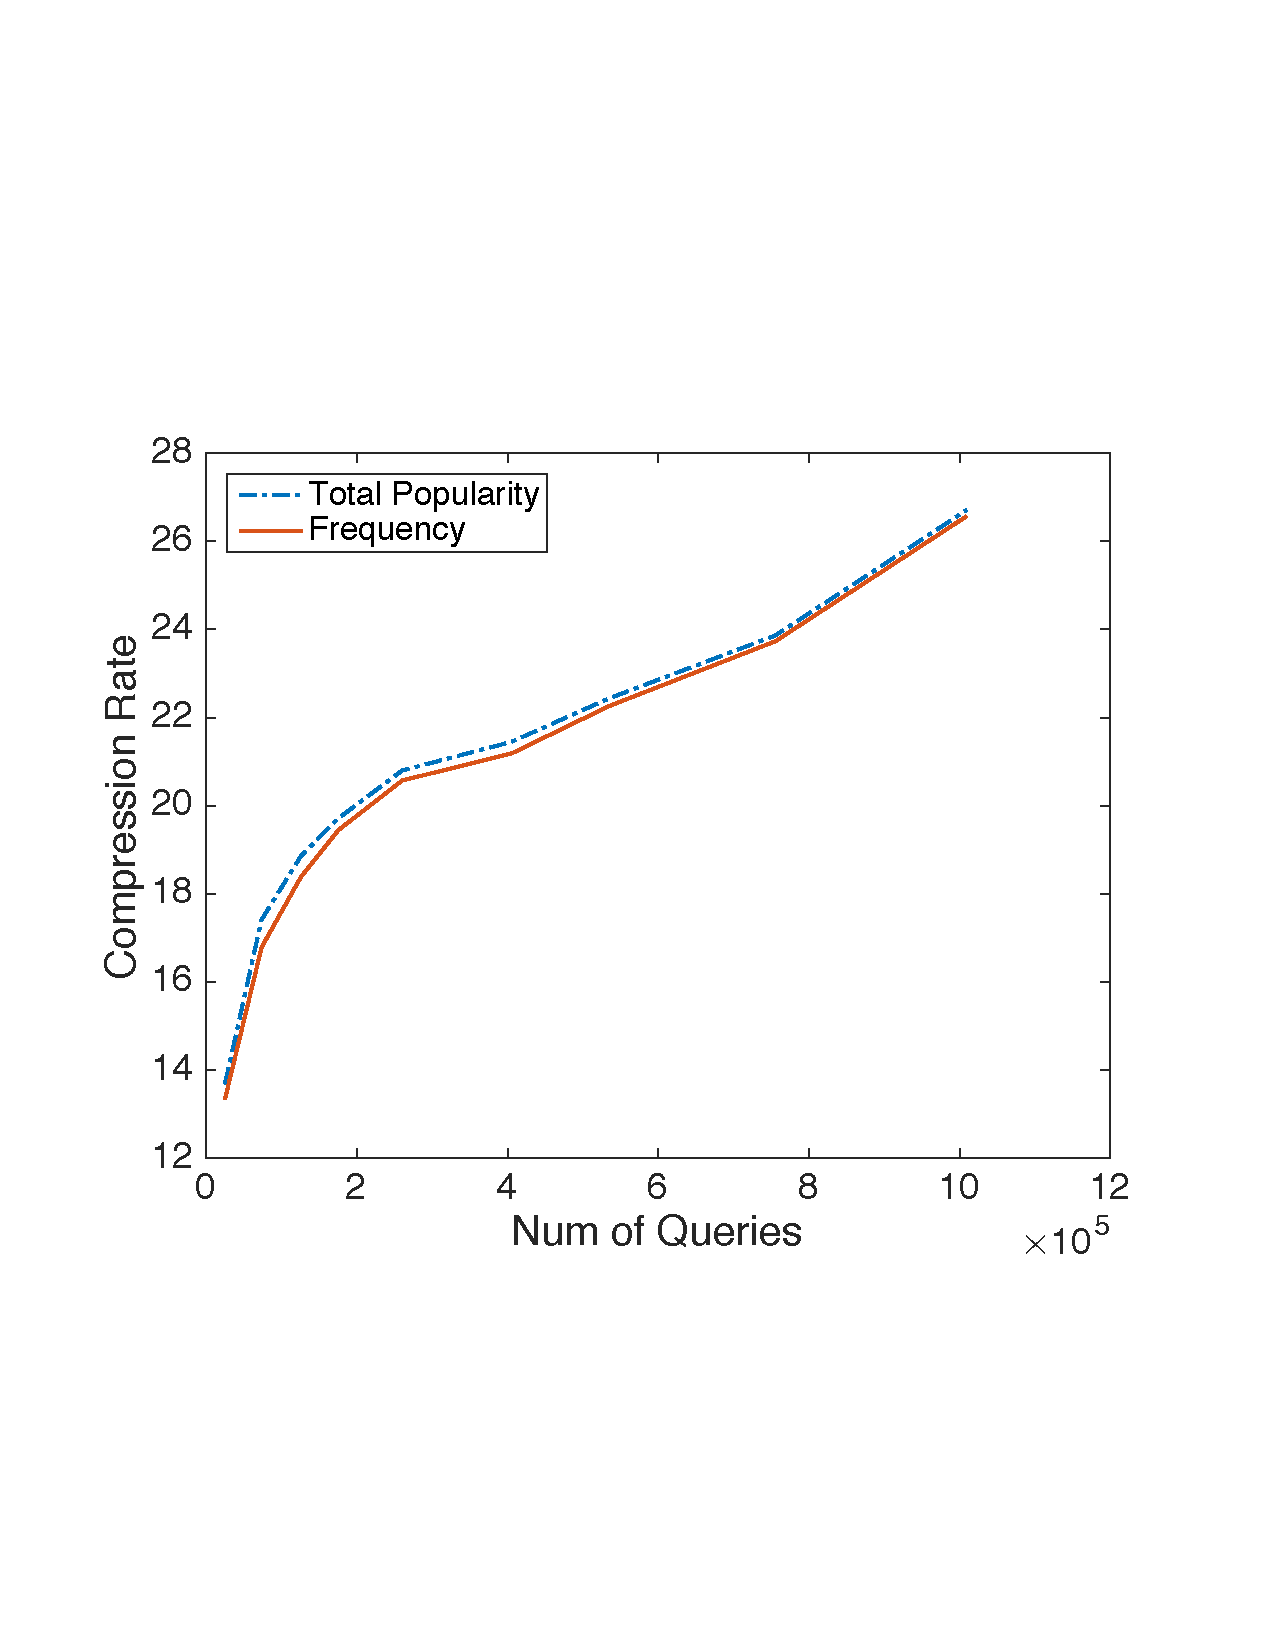
\includegraphics[height=5 cm]{graphics/compression_rate_scissored}
\caption{Comparison of compression rate of Total Popularity and Frequency in FP tree.}
\label{fig:compression_rate}
\end{figure}

The FP Tree structure provides a tree-like sub-clustering of queries that naturally tracks features common to queries in the sub-clusters.  Users can selectively traverse it by folding or unfolding subtrees to settle on an appropriate level of detail, without being overwhelmed.
Recall that each path from the root to a current visited node in the FP tree corresponds to a prefix of item sequences shared by real life queries. 
As the user traverses the tree, \sysname{} tries to reduce the length of the prefix by assembling its underlying feature ASTs and ideally creates a single assembly AST with updated multiplicity as the summary. In practice, the resulting summary is a set of assembly ASTs and we would like to improve readability by reducing the set size. Further expanding and visualizing an FP Tree is as intuitive as simply merging more feature AST components to the existing assembly AST. 

\begin{figure*}[h!]
\centering
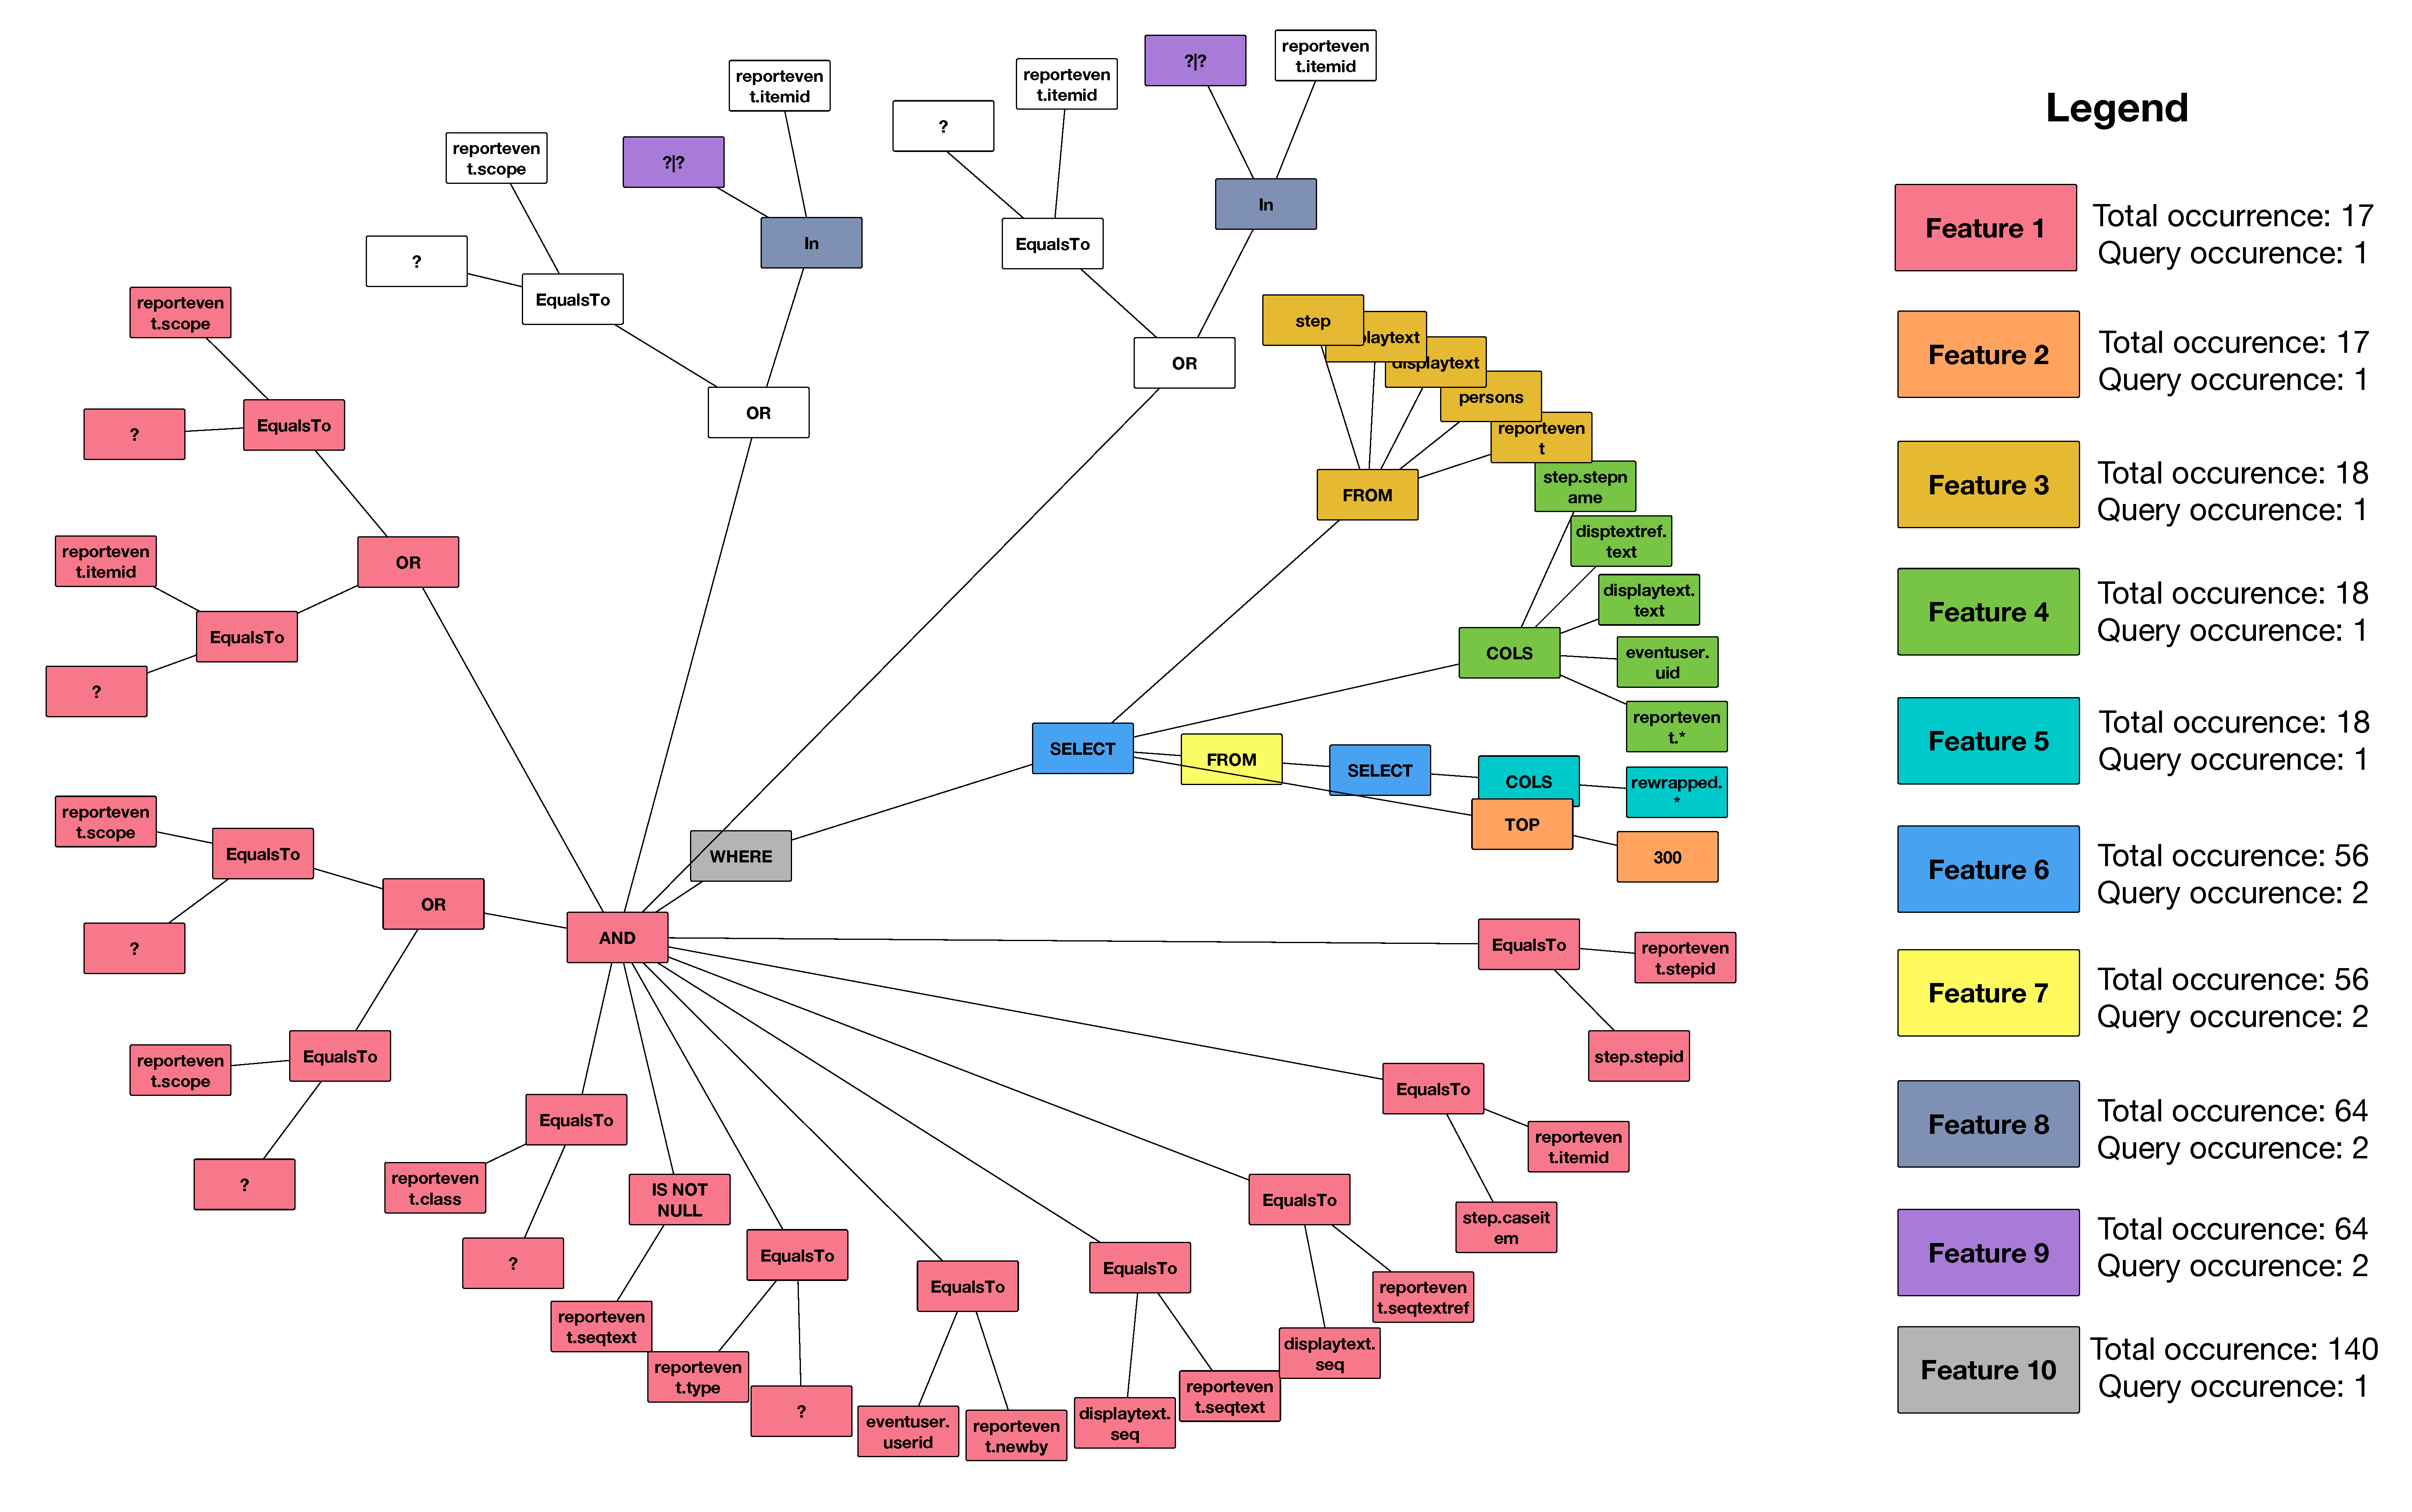
\includegraphics[height=11.5 cm]{graphics/exampleFPTreeColored}
%\caption{The common features identified and ranked in the summarization process is colored in the graph representing an AST, and the uncolored nodes are interchangeable.
\caption{An example AST of a SQL query where the common features that appears in all queries in the query group are colored and the uncolored nodes are specific only to that query.
}
\label{fig:summary_ast}
\end{figure*}

In general, reducing the set size contains two steps: (1) Shrink and (2) Merge.  The shrink step removes redundant items from the set as a preparation for merge step. Recall that an item $I$ is of the form $\tuple{f,mult_Q(f)}$. Given a specific feature $f_c \in \biguplus_{N \in Q}\featuresof{N}$, the set $S_c$ is defined as $$\comprehension{\tuple{f_p, mult_Q(f_p)}}{\astof{f_c} \subset \astof{f_p}, f_p \in \biguplus_{N \in Q}\featuresof{N}}$$ covers all items in the bag whose $\astof{f_p}$ fully contains $\astof{f_c}$. For any item $I_p=\tuple{f_p, mult_Q(f_p)} \in S_c$, suppose $f_c$ occurs $m_c$ times in the AST of feature $p$, by viewing item $I_p$, the inspector has already been informed of feature $f_c$ ($mult_Q(f_p)*m_c$) number of times. If we sum this for all $I_p \in S_c$ and compare the sum with the multiplicity of feature $f_c$, namely if $mult_Q(f_c) < \sum_{I_p\in S_c} mult_Q(f_p)*m_c$, item $I_c$ can be safely removed as redundant. Example \ref{shrink} shows a simple case of shrink.
\begin{example}
\label{shrink}
Consider a feature $f$ that encodes the expression $A=B$ with multiplicity 2, $\tuple{f,2}$. Consider another 2-tuple $\tuple{f',1}$ in the same feature bag which encodes $A=$ with multiplicity 1. It is possible that the multiplicity of $A=$ is less than $A=B$ as it is not necessary that each subgraph of $A=B$ is included in the bag. By viewing $A=B$ two times, the inspector is already informed of the existence of $A=$ structure two times which renders $\tuple{f',1}$ redundant.
\end{example}

Merge step further reduces the set size by a sequence of pairwise merge operation on items. Merge of two items is not merely the merge of their feature ASTs. The order of merge operations and the difference in feature multiplicity between two items should be carefully taken care of. In fact, the correctness of merge step needs to be verified by counting the number of original queries that share the resulting set of ASTs. This count should match with the count of queries, recorded in the FP Tree, that pass the chosen prefix.

In practice, shrink step is much faster and reliable than merge step: to guarantee the correctness of merge step, verification back on the original queries is required while shrink only involves local comparison on subtrees. In some cases that shrink step already produces minimal set size, merge step can be skipped.

Thus we recommend a property called \textit{Seal} for feature bags. Part of its goal is skipping merge step.
\begin{definition}
Property: Seal

Generic Seal: At least the complete subtree rooted at each node in the AST should be encoded as a feature; 

Tailored Seal: For any pair of distinct features in the feature bag of $Q$, if they assemble to $\astof{asmbly}$ which is also contained in query AST of $Q$, then structure $\astof{asmbly}$ should be included in the feature bag for $Q$.
\end{definition}
Generic Seal guarantees that features generated fully reconstructs the original query AST. 
With Tailored Seal, merge step can be skipped and features that encode assembly trees described in Tailored Seal are kept for summarization. Thus we are capable of providing the inspector a quick and a concise summary. It comes with the cost that depending on the number of additional features created, Seal would affect the scalability of \sysname{} with respect to memory consumption of FP Tree and speed of clustering. It may also affect clustering result as it changes the feature vector. Measuring and understanding the overall effect of applying property Seal are left for future work.

%\texttt{
%SELECT rewrapped.* FROM (SELECT TOP 300 reportevent.*, eventuser.uid AS uid, displaytext.text AS shortdesc, disptextref.text AS textref, step.stepname AS stepname FROM reportevent LEFT JOIN persons AS eventuser ON eventuser.userid = reportevent.newby LEFT JOIN displaytext AS displaytext ON displaytext.seq = reportevent.seqtext LEFT JOIN displaytext AS disptextref ON disptextref.seq = reportevent.seqtextref LEFT JOIN step AS step ON step.caseitem = reportevent.itemid AND step.stepid = reportevent.stepid WHERE ((reportevent.itemid IN ('') AND reportevent.scope = '') OR (reportevent.itemid = '' AND reportevent.scope = '')) AND reportevent.class = '' AND (reportevent.seqtext IS NOT NULL) AND reportevent.type = '' ORDER BY reportevent.eventid DESC) rewrapped ORDER BY rewrapped.eventid
%}
Figure~\ref{fig:summary_ast} shows an example AST resulting from a rule that only encodes the parental relationship between any node in query AST and the whole subtree rooted at one of its child node.
The AST is generated from a query and summarization information of the query set that it belongs to.
The 10 features shown with colored nodes appears at least once in every query in the query set. The legend shows that how many times the feature appears in all queries as ``Total occurrence", and in the example query itself as ``Query occurrence."
What makes this query different from the other ones is the uncolored nodes.
They either don't appear in the other queries, or appear infrequently.
This visualization makes a human inspector's work easier to spot important features and understand what the queries in the groups do, and identify why a query is different from the other queries.

%\subsection{Interesting Finding: An Induced Clustering Method}
%We propose an alternative clustering method that is induced by the summarization tree structure and claim that it has at least two advantages over existing clustering methods: (1) features are weighted automatically and intelligently (2) clusters are more interpretable, visualizable and easier to be merged and split.  

%From another perspective, a \textit{rooted path} summarizes a set of strings into a cluster and a sub-path can be viewed as its parent cluster. The whole tree is thus turned into a hierarchy of clusters. Nodes with various Height in the tree act as sub-cluster splitters and a node whose contained feature that is ranked higher in the ordering will execute its splitting job before that of a lower ranked one. This translates into the fact that total popularity of a feature is equivalent to its weight in a weight-assigned metric for measuring feature vector distance. A feature ranked higher by its popularity will enjoy a dominantly higher weight such that any discrepancy between the values of this feature will be enough to put two queries into different sub-clusters before the lower ranked feature is ever taken into consideration.

%\begin{example}
%The paths of all Select queries in the tree are guaranteed to start with feature 'SELECT' . The query without 'SELECT', no matter how similar the rest of its structure is to some Select query, will create new branch when trying to match the highest ranked 'SELECT' node in the tree and thus be put into a different cluster. This reflects that it is not a Select query. Intuitively, 'SELECT' is a characteristic feature of the whole set of Select queries and should be weighted so high that any discrepancy on it would cause enough increase in distance measure such that queries without it lead to different clusters.
%\end{example}

%Since paths that act as cluster representatives are guaranteed to maintain the syntactic correctness of its reconstructed partial AST and a visualization tool is provided.  It is much easier for human inspectors to visualize and interpret the induced cluster's shared intent and subsequently merge and split clusters. 

%\subsection{Boolean Formula Normalization}
%We transform all composite boolean formula in the query into Conjunctive Normal Form (CNF) as an intermediate step before feature generating process. 
%The logic behind is:
%(1) Queries with algebraically equivalent boolean formula share the same intent. Hence we need CNF  to reduce the whole algebraic equivalence class of formula into a uniform representation that reveals the shared intent;
%(2) No matter how complex the formula is, its CNF form, when translated into tree structure, has only Height three.  We benefit from CNF by restricting the Height of the corresponding tree structure hence greatly reducing the dimension of the feature vector in clustering step;
%(3) we use CNF instead of DNF because it is more sensitive to OR operators which in most cases are preferred by potential attackers to piggyback additional information
%\begin{example}
%A=a AND B=b is already in its CNF form while piggybacking OR C=c to it will dramatically change its corresponding CNF representation which becomes (A=a OR C=c) AND (B=b OR C=c).
%\end{example}

%\subsection{Online Monitoring}
%
%A third benefit of this approach to summarization is that the annotated clusters can also be used to construct a pattern-based classifier.  This is critical for one our motivating application of insider threat detection, as the number of queries processed by a typical corporate database is often too much for logging infrastructures to handle in the long term.  
%
% that can quickly group new queries into each of the three categories given in Section~\ref{sec:clustering}.  The matcher is run on queries as they arrive at the target database, enabling rapid response to potential threats. In the ideal case, we would be able to include each query in our considerations for the future queries, so we wouldn't need perform clustering in order to keep our system up to date. This approach is similar to the idea of database cracking~\cite{Stratos2007Cracking} suggesting that every query is a suggestion for the ideal structure of the database. By doing so, the maintenance becomes a byproduct of query validation process in order to avoid performing clustering repeatedly.
%
%
